\documentclass{beamer}
\usepackage[utf8]{inputenc}
\usepackage[czech]{babel}
\usepackage[T1]{fontenc}

\usetheme{Boadilla}
\usecolortheme{dolphin}

\title[algorithms]{Vizualizace třídicích algoritmů}
\author{Mykhailo Klunko}
\titlegraphic{
\includegraphics[scale=3]{Images/UPOL}}
\institute[UP]{Vedoucí: Mgr. Tomáš Kühr, Ph.D.\\
				Univerzita Palackého v Olomouci}
\date{\today}

\usepackage{listings}
\usepackage{listings}
\usepackage{color}

\definecolor{solarized@base03}{HTML}{002B36}
\definecolor{solarized@base02}{HTML}{073642}
\definecolor{solarized@base01}{HTML}{586e75}
\definecolor{solarized@base00}{HTML}{657b83}
\definecolor{solarized@base0}{HTML}{839496}
\definecolor{solarized@base1}{HTML}{93a1a1}
\definecolor{solarized@base2}{HTML}{EEE8D5}
\definecolor{solarized@base3}{HTML}{FDF6E3}
\definecolor{solarized@yellow}{HTML}{B58900}
\definecolor{solarized@orange}{HTML}{CB4B16}
\definecolor{solarized@red}{HTML}{DC322F}
\definecolor{solarized@magenta}{HTML}{D33682}
\definecolor{solarized@violet}{HTML}{6C71C4}
\definecolor{solarized@blue}{HTML}{268BD2}
\definecolor{solarized@cyan}{HTML}{2AA198}
\definecolor{solarized@green}{HTML}{859900}

\lstdefinestyle{solarized-light}
{
	basicstyle=\footnotesize\ttfamily\color{solarized@base00},
	backgroundcolor=\color{solarized@base3},
	rulesepcolor=\color{solarized@base3},
	numberstyle=\tiny\color{solarized@base1},
	keywordstyle=\color{solarized@green},
	stringstyle=\color{solarized@cyan}\ttfamily,
	identifierstyle=\color{solarized@blue},
	commentstyle=\color{solarized@base1},
	emphstyle=\color{solarized@red},
}

\lstdefinestyle{solarized-dark}
{
	basicstyle=\footnotesize\ttfamily\color{solarized@base01},
	backgroundcolor=\color{solarized@base03},
	rulesepcolor=\color{solarized@base03},
	numberstyle=\tiny\color{solarized@base01},
	keywordstyle=\color{solarized@green},
	stringstyle=\color{solarized@cyan}\ttfamily,
	identifierstyle=\color{solarized@base0},
	commentstyle=\color{solarized@base01},
	emphstyle=\color{solarized@red},
}

\lstset
{
	basicstyle=\footnotesize,        % Styl a typ písma
	captionpos=b,                    % Pozice popisku
	showstringspaces=false,          % Když true, místo mezer se vypíše podtržítko. e.g. "Hello_world"
	tabsize=4,                       % Velikost tabulátoru (počet mezer)
	style=solarized-dark,
	literate=
		{á}{{\'a}}1     {í}{{\'i}}1     {é}{{\'e}}1
		{ý}{{\'y}}1     {ú}{{\'u}}1     {ó}{{\'o}}1
		{ě}{{\v{e}}}1   {š}{{\v{s}}}1   {č}{{\v{c}}}1
		{ř}{{\v{r}}}1   {ž}{{\v{z}}}1   {ď}{{\v{d}}}1
		{ť}{{\v{t}}}1   {ň}{{\v{n}}}1   {ů}{{\r{u}}}1
		{Á}{{\'A}}1     {Í}{{\'I}}1     {É}{{\'E}}1
		{Ý}{{\'Y}}1     {Ú}{{\'U}}1     {Ó}{{\'O}}1
		{Ě}{{\v{E}}}1   {Š}{{\v{S}}}1   {Č}{{\v{C}}}1
		{Ř}{{\v{R}}}1   {Ž}{{\v{Z}}}1   {Ď}{{\v{D}}}1
		{Ť}{{\v{T}}}1   {Ň}{{\v{N}}}1   {Ů}{{\r{U}}}1
	,
}

\newcommand{\separator}{\vspace{15pt}}

\begin{document}

	\begin{frame}
		\titlepage
	\end{frame}

	\begin{frame}{Cíle práce}
		Požadavky:
		\begin{itemize}
			\item Vytvořit software pro podporu výuky třídících algoritmů pomocí vizualizace průběhu třídění
			\item Podpora nejznámějších algoritmů
			\item Vizualizace algoritmů na zadaném či vygenerovaném vstupním poli
			\item Krokování průběhu výpočtu 
			\item Zobrazení pseudokódu použitého algoritmu a aktuálních hodnot proměnných
		\end{itemize}
	\end{frame}

	\begin{frame}{Problém}
	Podpora výuky třídících algoritmů:
		\begin{enumerate}
			\item Pochopení algoritmů
			\item Průběh třídění
		\end{enumerate}
	\end{frame}


	\begin{frame}{Použité technologie}
		\begin{itemize}
			\item Java
			\item JavaFX
			\item CSS
		\end{itemize}
	\end{frame}

	\begin{frame}{Java}
		\begin{itemize}
			\item Cross-platform
			\item Program nevyužívá velky objem paměti
		\end{itemize}
		\begin{center}
			
\includegraphics[scale=0.2]{Images/java}
		\end{center}
		
	\end{frame}

	\begin{frame}{Ukázka}
		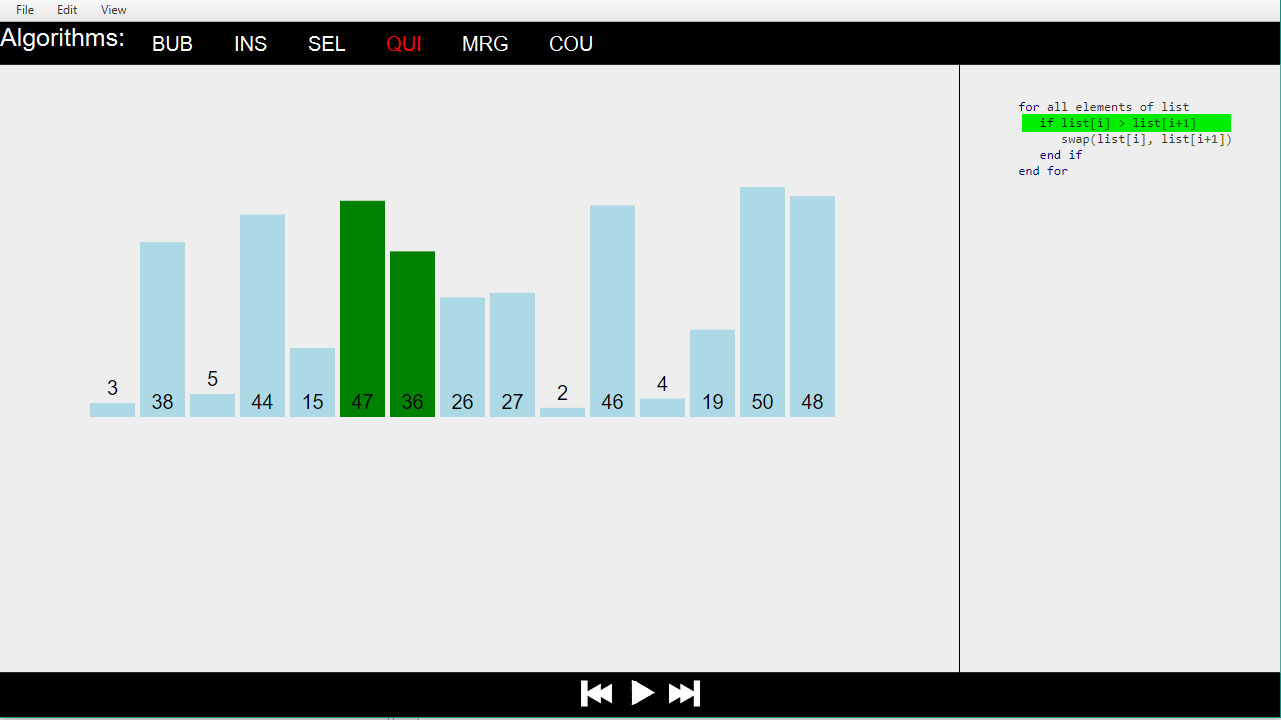
\includegraphics[scale=0.35]{Images/Demo}
	\end{frame}

	\begin{frame}{Závěr}
		Odkazy:
		\begin{itemize}
			\item http://docs.oracle.com/en/java/
		\end{itemize}
		\vspace{70pt}
		\centerline{\textbf{Děkuji za pozornost.}}
	\end{frame}

\end{document}